\documentclass{article}

% use package to control paper dimensions
\usepackage{geometry}
 \geometry{
		a4paper,
		% left=22mm,
		% right=22mm,
		top=20mm,
		bottom=20mm
}

% Add 'authorblk' package for affliation support
\usepackage{authblk}

% Add package mathbb, amsmath for mathematical symbols and equation
\usepackage{amsmath}
\usepackage{amssymb}
\newcommand{\R}{\mathbb{R}}

% Add package 'graphicx' for figures
\usepackage{graphicx}

% use packages for code listings
\usepackage{listings}
\usepackage{color}
\usepackage{xcolor}

\definecolor{mGreen}{rgb}{0,0.6,0}
\definecolor{mGray}{rgb}{0.5,0.5,0.5}
\definecolor{mPurple}{rgb}{0.58,0,0.82}
\definecolor{CBackgroundColour}{rgb}{0.95,0.95,0.92}

\usepackage{caption}
\DeclareCaptionFont{white}{\color{white}}
\DeclareCaptionFormat{listing}{\colorbox{gray}{\parbox{0.98\textwidth}{#3}}}
\captionsetup[lstlisting]{format=listing,labelfont=white,textfont=white}

\lstdefinestyle{CStyle}{
    backgroundcolor=\color{CBackgroundColour},   
    commentstyle=\color{mGreen},
    keywordstyle=\color{magenta},
    numberstyle=\tiny\color{mGray},
    stringstyle=\color{mPurple},
    basicstyle=\footnotesize,
    breakatwhitespace=false,         
    breaklines=true,                 
    captionpos=t,                    
    keepspaces=true,                 
    showspaces=false,                
    showstringspaces=false,
    showtabs=false,                  
    tabsize=2,
    language=C
}

\definecolor{BashBackgroundColour}{rgb}{0.7,0.7,0.7}
\lstdefinestyle{BashStyle}{
    basicstyle=\small\ttfamily,
    breaklines=true,                 
    language=bash
}

% Use package 'hyperref' for hyperlink references
\usepackage{hyperref}

\usepackage{multirow}

\usepackage{subcaption}

\usepackage{dirtree}

\usepackage[title]{appendix}

% Title, author and affliations related headers of article
\title{Analyzing the Parallelizablity of SVM Classification Algorithm using OpenMP}
\author{R Mukesh (CED15I002)}
\affil{IIITDM Kancheepuram}

\date{}

\begin{document}
\maketitle

\begin{abstract}
Support Vector Machine (SVM) is among the most popular algorithms in machine learning literature. This paper aims to analyze the performance of parallelized SVM classification algorithm using OpenMP.
\end{abstract}

\section{Theory}

	\subsection{Overview of Support Vector Machines}
	
		Consider a binary classification dataset,
			\[
				\{(x^{(i)}, y^{(i)})\ |\ i=1, \ldots, m\}
			\]			
		
		where, 	$x^{(i)} \in \R^n$ is the feature vector representing i\textsuperscript{th} training instance.\par
		\hspace{32pt}$y^{(i)} \in \{-1, 1\}$ is the class label corresponding to i\textsuperscript{th} training instance.\par
		
		\begin{figure}[!htbp]
			\centering
			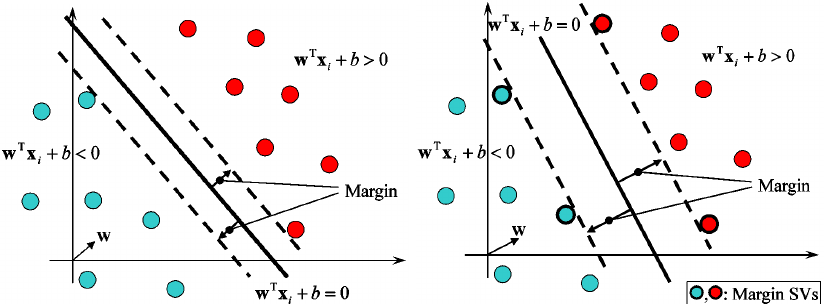
\includegraphics[scale=0.4]{svm}
			\caption{Optimal margin linear seperating hyperplane.}
		\end{figure}
		
		The SVM learning algorithm learns the parameters ($w$, $b$) of the optimal margin linear seperating hyperplane (for the data transformed to an higher dimensional feature space using the kernel trick).
		
		Maximizing the margin of the linear seperating hyperplane can be expressed as an constrained optimization problem:
		
		\begin{equation*}
			\begin{aligned}
				& \underset{w, b}{minimize}
				& & \frac{1}{2} ||w||^2 \\
				& \text{subject to}
				& & y^{(i)}(w^Tx^{(i)}+b) \geq 1, \; i = 1, \ldots, m.
			\end{aligned}
		\end{equation*}
		
		Using the langragian, the dual form of the optimization is formulated as a quadratic programming problem:
		
		\begin{equation*}
			\begin{aligned}
				& \underset{\alpha}{maximize}
				& & \Psi(\alpha) = \sum_{i=1}^{m} \alpha_i - \frac{1}{2} \sum_{i,j=1}^{m} y^{(i)} y^{(j)} \alpha_i \alpha_j \langle x^{(i)}, x^{(j)} \rangle \\
				& \text{subject to}
				& & \alpha_i \geq 0, \; i=1, \ldots, m. \\
				& & & \sum_{i=1}^{m} \alpha_i y^{(i)} = 0								
			\end{aligned}					
		\end{equation*}
		
		The parameter $w$ that characterizes the optimal margin linear seperating hyperplane is computed:
		
		\begin{equation*}
			w = \sum_{i=1}^{m} \alpha_i y^{(i)} x^{(i)}
		\end{equation*}
				
		To make the algorithm work for non-linearly seperable datasets as well as less sensitive to outliers, we reformulate the optimization (using ${\textbf l_1}$ regularization):
		
		\begin{equation}
			\label{regularised_dual_form}
			\begin{aligned}
				& \underset{\alpha}{maximize}
				& & \Psi(\alpha) = \sum_{i=1}^{m} \alpha_i - \frac{1}{2} \sum_{i,j=1}^{m} y^{(i)} y^{(j)} \alpha_i \alpha_j \langle x^{(i)}, x^{(j)} \rangle \\
				& \text{subject to}
				& & 0 \leq \alpha_i \leq C, \; i=1, \ldots, m. \\
				& & & \sum_{i=1}^{m} \alpha_i y^{(i)} = 0 \\
				& & & \text{where, \textbf{C} is the regularization parameter.}
			\end{aligned}					
		\end{equation}		
		
		The Karush-Kuhn-Tucker(KKT) conditions are necessary and sufficient for the optimal value of a positive-definite quadratic programming problem. The KKT (or convergence) conditions for the quadratic programming problem (\ref{regularised_dual_form}) for $i=1, \ldots, m$ are:
		
		\begin{equation}
			\label{kkt_conditions}
			\begin{aligned}
				\alpha_i = 0 \iff y^{(i)} (w^T x^{(i)} + b) \geq 1 \\
				\alpha_i = C \iff y^{(i)} (w^T x^{(i)} + b) \leq 1 \\
				0 < \alpha_i < C \iff y^{(i)} (w^T x^{(i)} + b) = 1 \\
			\end{aligned}
		\end{equation}
		
	\subsection{The SMO Algorithm}
		
		Sequential Minimal Optimization (SMO) is an efficient algorithm to the solve the SVM quadratric programming problem in (\ref{regularised_dual_form}).
		
		\begin{quote}
			Repeat until convergence \{
				\begin{enumerate}
					\item Choose a pair of langrage multipliers $\alpha_i, \alpha_j$ to jointly optimize (using an heuristic that maximizes the size of step in optimizing $\Psi(\alpha)$).
					\item If the choosen pair of langrage multipliers $\alpha_i, \alpha_j$ can make a positive step in optimizing $\Psi(\alpha)$, reoptimize $\Psi(\alpha)$ with respect to $\alpha_i, \alpha_j$, while holding all other $\alpha_k s(k \neq i,j)$ fixed.
				\end{enumerate}
			\}
			
			For convergence, the KKT conditions in (\ref{kkt_conditions}) must be satisfied for all $\alpha_i s$.
		\end{quote}
		
\section{Parallelizing the SMO Algorithm}
	
	\textbf{Sequential} Minimal Optimization (SMO) is an \textbf{iterative} optimization algorithm and the scope for parallelization is limited. The operations involved in an iteration of the optimization (such as searching $\alpha_i, \alpha_j$ pair to update and updating error between predicted and actual value for each training instance) can be performed parallely:
	
	\begin{enumerate}
		\item{\textbf{Initializing and updating error cache for each training instance:}} \par
		In each update of an $\alpha_i, \alpha_j$ pair, the $w$ and $b$ paramters of the model are also updated. Consequentially, the error cache that represents the difference between the model's predicted and actual value for each training instance is updated parallely.
		
		The update of the error cache for each training instance was parallelized using the OpenMP construct:\lstinline[style=CStyle]{#pragma omp parallel for}.
		
		\begin{lstlisting}[style=CStyle]					
			#pragma omp parallel for private(i)
			for(i = 0; i< m; ++i)
			{
			
				Initialize or update error cache for the ith training instance
				
			}
		\end{lstlisting}
		
		\item {\textbf{Searching across $\alpha_i, \alpha_j$ pairs for one that can make positive step in optimizing the objective $\Psi(\alpha)$}:} \par
		Pairs of $\alpha_i, \alpha_j$ are parallely tested until a pair is found that can be updated to make positive step in optimizing the problem in (\ref{regularised_dual_form}). Consequentially, the time taken to find the $\alpha_i, \alpha_j$ pair to update and thereby the time taken for the convergence of the SMO algorithm are drastically reduced.
		
		The searching of the $\alpha_i, \alpha_j$ pair to update was parallelized using the OpenMP constructs: \lstinline[style=CStyle]{#pragma omp parallel for}, \lstinline[style=CStyle]{#pragma omp critical}, \lstinline[style=CStyle]{#pragma omp cancel for}, \lstinline[style=CStyle]{#pragma omp cancellation point for}, and using private and shared thread syncronization variables.
		
		\begin{lstlisting}[style=CStyle]	
						
			Find an alpha[i] that violates the KKT-conditions
	
			// shared sync var to indicate success in finding alpha pair to update			
			valid_alphaj_found = false;
						
			#pragma omp parallel
			{
				#pragma omp for priavte(j)
				for(j=0; j<m; ++j)
				{
					#pragma omp cancellation point for
					
					if((i != j) && (valid_alphaj_found == false))
						if(alpha[i], alpha[j] can make positive step in optimization)
						{
							// local sync var to indicate success in finding alpha pair to update by this iteration
							bool thread_valid_alphaj_found = false;
							
							#pragma omp critical
							{							
								if(valid_alphaj_found == false)
								{
									valid_alphaj_found = true;
									thread_valid_alphaj_found = true;
									
									Update the alpha pair, model parameters and error cache
								}
							} // end of omp critical
							
							if(thread_valid_alphaj_found == true)
							{
								#pragma omp cancel for
							}
						}
				} // end of omp for
			} // end of omp parallel
			
			if vaid_alphaj_found became true
				a valid alpha[i], alpha[j] was found and updated
				
			else
				no such alpha[i], alpha[j] pair exists for the given alpha[i]
		\end{lstlisting}
		
		\item{\textbf{Computing dot product of feature vectors:}} \par
		The popularity of SVM can be largely attributed to the kernel trick that enables us find the optimal margin linear seperating hyperplane in a \textbf{higher dimensional feature space}. The kernel function (such as linear kernel) often involves the computation of the dot product of the the feature vectors.
		
		The computation of the dot product of the feature vectors can be parallelized using OpenMP construct: \lstinline[style=CStyle]{#pragma omp parallel for} with reduction.
		
		\begin{lstlisting}[style=CStyle]	
						
			dot_product = 0;
			
			#pragma omp parallel for private(i) reduction(+:dot_product)			
			for(i=0; i<n; ++i)
				dot_product += feature_vector1[i] * feature_vector2[i];
				
		\end{lstlisting}
	\end{enumerate}
	
\section{Results \protect\footnote{The experiments were conducted on a computer with 6\textsuperscript{th} Generation Intel(R) Core(TM) i7-6500U Processor (4M Cache, upto 3.10 GHz) and 8GB Single Channel DDR3L 1600M Hz (4GBx2) RAM.}}


	The experiments were performed on pre-processed excerpts of the \href{https://archive.ics.uci.edu/ml/datasets/adult}{Adult Data Set} from UCI Machine Learning Repository. The pre-processed training dataset \href{https://www.csie.ntu.edu.tw/~cjlin/libsvmtools/datasets/binary/a1a}{a1a} and testing dataset \href{https://www.csie.ntu.edu.tw/~cjlin/libsvmtools/datasets/binary/a1a.t}{a1a.t} can be downloaded from the \href{https://www.csie.ntu.edu.tw/~cjlin/libsvmtools/datasets/binary.html}{LIBSVM datasets page}.
	
	\begin{quote}
		\textbf{Number of classes  :} 2 \\
		\textbf{Number of data     :} 1,605 / 30,956 (testing) \\
		\textbf{Number of features :} 123 / 123 (testing)
	\end{quote}
	
	\begin{table}[!htbp]
	\begin{tabular}{|c|c|c|}
	\hline
	\multicolumn{1}{|l|}{\multirow{2}{*}{\textbf{Number of Threads}}} & \multicolumn{2}{c|}{\textbf{Execution Time (in seconds)}}                                                            \\ \cline{2-3} 
	\multicolumn{1}{|l|}{}                                            & \multicolumn{1}{l|}{\textbf{Fitting with training data}} & \multicolumn{1}{l|}{\textbf{Predicting for testing data}} \\ \hline
	1                                                                 & 1195.73                                                  & 24.0849                                                   \\ \hline
	2                                                                 & 604.719                                                  & 14.2085                                                   \\ \hline
	4                                                                 & 1589.9                                                   & 12.7448                                                   \\ \hline
	6                                                                 & 669.508                                                  & 14.2376                                                   \\ \hline
	8                                                                 & 598.881                                                  & 13.2541                                                   \\ \hline
	12                                                                & 582.259                                                  & 13.7397                                                   \\ \hline
	16                                                                & 740.158                                                  & 14.7316                                                   \\ \hline
	20                                                                & 1420.45                                                  & 15.2676                                                   \\ \hline
	24                                                                & 656.442                                                  & 16.0162                                                   \\ \hline
	28                                                                & 614.798                                                  & 17.0384                                                   \\ \hline
	32                                                                & 747.298                                                  & 18.5145                                                   \\ \hline
	\end{tabular}
	\end{table}
	
	The speed of convergence of the fitting of SVM model is dictated by the path taken (i.e., the choice of $\alpha_i, \alpha_j$ pairs at each iteration of the optimization algorithm). Since, the choice of $\alpha_i, \alpha_j$ pairs is partly random, the time taken for the convergence of the SVM fitting is likely to vary across runs.
	
	\begin{figure}[!htbp]

		\centering
		\begin{subfigure}[!htbp]{\textwidth}
			\centering
			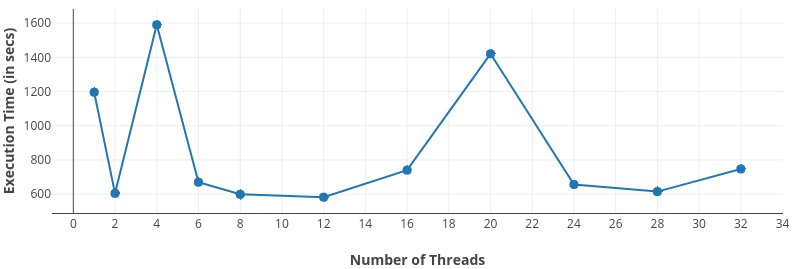
\includegraphics[scale=0.5]{fit_graph}
			\subcaption{Performance of the fit method in SVM learning algorithm}
		\end{subfigure}
		
		\begin{subfigure}[!htbp]{\textwidth}
			\centering
			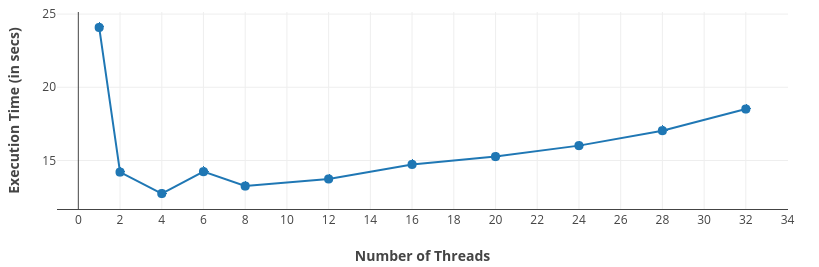
\includegraphics[scale=0.5]{predict_graph}
			\subcaption{Performance of the predict method in SVM learning algorithm}
		\end{subfigure}
	
		\caption{Number of Threads vs Execution Time for fit and predict methods of SVM learning algorithm in OpenMP}
	\end{figure}
	
\section{Calculation}

	The parallel fraction of the algorithm can be computed using the following equation:

	\begin{equation}
		f = \frac{(1-T_p/T_1)}{(1-1/p)}
	\end{equation}
	
	
	For Fit Method of SVM Learning Algorithm,
	\[
		f = \frac{(1-582.259/1195.73)}{(1-1/12)} = \textbf{0.559692482 (55.97 \%)}
	\]
	
	For Predict Method of SVM Learning Algorithm,
	\[
		f = \frac{(1-12.7448/24.0849)}{(1-1/4)} = \textbf{0.627784767 (62.78 \%)}
	\]
	
\section{Inferences}

	\begin{enumerate}
		\item The \textbf{fit and predict methods} of the parallelized SVM classification algorithm have parallel fractions of \textbf{55.97 \%} and \textbf{62.78 \%} respectively.
		
		\item The execution time of the fit method of the parallelized SVM classification algorithm varies significantly across runs (for a fixed number of threads) due to the randomness associated with the \textbf{path taken towards convergence}.
		
		\item The parallelization of dot product computation deteriorates the performance of the algorithm due to the limitations of the hardware and the \textbf{overhead} associated with creation and switching of threads.
		
	\end{enumerate}
\pagebreak

\begin{appendices}
	\section{Downloading and Running Source Code}
		\subsection{Downloading the Source Code}
			The source code of the parallel implementation of SMO algorithm in C++ using OpenMP can be downloaded \href{https://github.com/elixir-code/HPC-Lab/Project/SVM-OpenMP/svm-openmp-codes.zip}{\textbf{here}}. 
			
			Please visit the github repository \href{https://github.com/elixir-code/HPC-Lab/}{\textbf{elixir-code/HPC-Lab}} for supplementary resources.
			
		\subsection{Running the Source Code}
			\begin{enumerate}
				\item Extract the zip file containing the source code.				
					\begin{lstlisting}[style=BashStyle]
$ unzip <path to downloaded source code zip>/svm-openmp-codes.zip
					\end{lstlisting}
				
				\item Open the terminal and change the current directory to the extracted directory that contains source code.
					\begin{lstlisting}[style=BashStyle]
$ cd <path where source code zip was extracted>/svm-openmp-codes
					\end{lstlisting}
			
				\item Build the code using the make utility.
				\begin{lstlisting}[style=BashStyle]
$ make
			\end{lstlisting}
				
				This generates the intermediate object files and executables for the test programs.
				
				\item Execute the test program executable generated by the make script.
				
					For example: To run the sample test program '\textbf{test1.cpp}' located in the '\textbf{test}' directory.
					\begin{lstlisting}[style=BashStyle]
$ ./build/bin/test1
					\end{lstlisting}
					
					Write your own test programs using the functions defined in the header files in the '\textbf{include}' directory. Rebuild the code using the make utility and execute the generated test program executable located in '\textbf{build/bin}' directory.
			\end{enumerate}
	
	\pagebreak
		
	\section{Complete Source Code}
	
		Structure of the project:
		
		\dirtree{%
			.1 .
			.1 include.
			.2 dataset.hpp.
			.2 classifier.hpp.
			.2 kernel.hpp.
			.2 validation.hpp.			
			.1 src.
			.2 dataset.cpp.
			.2 classifier.cpp.
			.2 svm.cpp.
			.2 kernel.cpp.
			.2 validation.cpp.
			.1 test.
			.2 test1.cpp.
			.1 datasets.
			.2 a1a.
			.2 a1a.t.
		}
		
		\lstinputlisting[style=CStyle, caption={\textbf{include/dataset.hpp}}]{../svm-openmp-codes/include/dataset.hpp}
		\lstinputlisting[style=CStyle, caption={\textbf{include/classifier.hpp}}]{../svm-openmp-codes/include/classifier.hpp}
		\lstinputlisting[style=CStyle, caption={\textbf{include/kernels.hpp}}]{../svm-openmp-codes/include/kernels.hpp}
		\lstinputlisting[style=CStyle, caption={\textbf{include/validation.hpp}}]{../svm-openmp-codes/include/validation.hpp}
		
		\lstinputlisting[style=CStyle, caption={\textbf{src/dataset.cpp}}]{../svm-openmp-codes/src/dataset.cpp}
		\lstinputlisting[style=CStyle, caption={\textbf{src/classifier.cpp}}]{../svm-openmp-codes/src/classifier.cpp}
		\lstinputlisting[style=CStyle, caption={\textbf{src/svm.cpp}}]{../svm-openmp-codes/src/svm.cpp}
		\lstinputlisting[style=CStyle, caption={\textbf{src/kernels.cpp}}]{../svm-openmp-codes/src/kernels.cpp}
		\lstinputlisting[style=CStyle, caption={\textbf{src/validation.cpp}}]{../svm-openmp-codes/src/validation.cpp}
		
		\lstinputlisting[style=CStyle, caption={\textbf{test/test1.cpp}}]{../svm-openmp-codes/test/test1.cpp}
		
	
\end{appendices}
		
		
\end{document}